\documentclass[conference]{IEEEtran}
\usepackage{cite}
\usepackage{amsmath,amssymb,amsfonts}
\usepackage{algorithmic}
\usepackage{graphicx}
\usepackage{textcomp}
\usepackage{xcolor}
\usepackage{booktabs}
\usepackage{tabularx}
\usepackage{array}
\usepackage{float}
\usepackage{url}
\usepackage{multirow}
\usepackage{bm}

\begin{document}

\title{Advanced Hyperspectral Image Analysis in Precision Agriculture and Land Cover Mapping through Optimized Self-Modulating Convolutional Neural Networks}

\author{
\IEEEauthorblockN{1\textsuperscript{st} Swati Hira}
\IEEEauthorblockA{\textit{Dept. of Computer Science and} \\
\textit{Engineering} \\
\textit{IIIT Nagpur} \\
Nagpur, India \\
shira@iiitn.ac.in}
\and
\IEEEauthorblockN{2\textsuperscript{nd} Devguru Tiwari}
\IEEEauthorblockA{\textit{Dept. of Computer Science and} \\
\textit{Engineering} \\
\textit{IIIT Nagpur} \\
Nagpur, India \\
bt23csd060@iiitn.ac.in}
}

\maketitle

% ============================================================
% ABSTRACT
% ============================================================
\begin{abstract}
Hyperspectral image (HSI) classification is fundamental to precision agriculture and land cover mapping, yet conventional convolutional neural networks (CNNs) apply static learned filters uniformly across all spectral-spatial inputs, ignoring the significant variation in spectral signatures across diverse land cover types. We propose the \textbf{Self-Modulating Convolutional Neural Network (SMCNN)}, which incorporates \textbf{Spectral Self-Modulating Residual Blocks (SSMRB)}-a domain-specific adaptation of affine feature modulation for hyperspectral imagery that dynamically adjusts convolutional feature responses based on the input's spectral context. Building on affine feature modulation principles (FiLM, SE-Net), SSMRB generates both scaling ($\gamma$) and shifting ($\beta$) parameters, enabling input-dependent feature recalibration within residual blocks. Rather than claiming a fundamentally new architecture, we present an empirical investigation into how this specific combination impacts spectral feature learning.

Our pipeline integrates: (i)~\textbf{Adaptive Spectral Wiener Denoising (AWP)} for noise-robust preprocessing, (ii)~\textbf{Wavelet Spectral Augmentation (WFA)} for multi-scale spectral feature expansion via DWT decomposition, and (iii)~the \textbf{SMCNN} classifier with SSMRB.

We evaluate on \textbf{six benchmark HSI datasets}-Indian Pines, Pavia University, Salinas, Botswana, Kennedy Space Center, and WHU-Hi HanChuan-reporting: \textbf{96.17 $\pm$ 0.25\% OA} on Indian Pines (95\% CI: [95.86, 96.48]), \textbf{99.47 $\pm$ 0.04\% OA} on Pavia University, and \textbf{98.59 $\pm$ 0.87\% OA} on Botswana. The addition of $\beta$ is consistently associated with improved \textbf{Average Accuracy (AA)} on minority classes (e.g., +5.36\% AA over Plain 2D-CNN on Indian Pines), with only \textbf{0.19M parameters} and 10--22$\times$ faster training than transformer baselines, though we note that formal statistical significance testing is limited by our 5-seed experimental design, the causal mechanism of $\beta$'s effect has not been directly verified, and the 2D-CNN architecture struggles on highly overlapping wetland ecosystems (KSC) where 3D transformers remain strictly superior.
\end{abstract}

\renewcommand\IEEEkeywordsname{Keywords}
\begin{IEEEkeywords}
Hyperspectral Image Classification, Self-Modulating CNN, Spectral Self-Modulation, Affine Feature Modulation, Precision Agriculture, Wavelet Spectral Augmentation, Land Cover Mapping
\end{IEEEkeywords}

% ============================================================
% I. INTRODUCTION
% ============================================================
\section{Introduction}

\subsection{Problem Statement}

Hyperspectral imaging captures hundreds of contiguous spectral bands across the electromagnetic spectrum, providing rich spectral signatures that enable fine-grained discrimination between visually similar land cover types. However, HSI classification faces three fundamental challenges:

\begin{enumerate}
\item \textbf{High dimensionality}: Hundreds of spectral bands create the Hughes phenomenon (curse of dimensionality)~\cite{hughes1968mean}, where classifier performance degrades as feature space grows faster than available training samples.
\item \textbf{Spectral noise and atmospheric interference}: Sensor noise, atmospheric absorption, and calibration artifacts corrupt spectral signatures, particularly in water-absorption bands.
\item \textbf{Mixed pixels and spectral variability}: At typical spatial resolutions (1--30~m), individual pixels often contain mixtures of multiple land cover types, and the same material can exhibit significant spectral variation across different conditions.
\end{enumerate}

\subsection{Limitations of Existing Approaches}

Standard CNNs apply the same learned convolutional filters to all inputs regardless of their spectral content. This static behavior is suboptimal for HSI data where different crop types activate fundamentally different spectral regions, the optimal feature emphasis varies significantly between vegetation (NIR-sensitive) and urban materials (SWIR-sensitive), and local noise characteristics vary across spectral bands.

\subsection{Contributions}

This paper asks: \textit{does adding a learned shift parameter $\beta$ alongside channel scaling $\gamma$ improve HSI classification, and if so, which classes benefit most?} The building blocks-affine modulation (FiLM~\cite{perez2018film}), channel attention (SE-Net~\cite{hu2018squeeze}), residual learning (ResNet~\cite{he2016deep})-are fully established. Our contribution is not a novel mathematical mechanism, but rather a systematic empirical study of this configuration in the spectral domain:

\begin{enumerate}
\item \textbf{An empirical finding}: Adding $\beta$ reverses the AA$-$OA gap from $-$1.34 (baseline) to +2.05, while scale-only modulation (SE-Net) only reduces it to $-$0.42 (Section~\ref{sec:senet_ablation}). This pattern-observed on both tested datasets-suggests that $\beta$ preferentially aids minority classes, a finding relevant to precision agriculture where rare crop identification matters.
\item \textbf{Systematic evaluation}: We evaluate SSMRB under HSI-specific constraints (5\% training split, 103--274 bands, four sensor types, six datasets) with full ablation, noise robustness, and interpretability analysis.
\item \textbf{Practical efficiency}: SMCNN achieves accuracy competitive with transformers on 2/4 datasets at 10--22$\times$ lower training cost with 0.19M parameters, demonstrating that lightweight modulated CNNs remain viable under data-scarce conditions.
\end{enumerate}

\subsection{Pipeline Rationale}

The preprocessing pipeline follows a principled sequence: AWP (Adaptive Wiener Preprocessing) applies band-adaptive Wiener filtering to suppress sensor noise, producing smoothed spectra. However, denoising necessarily attenuates high-frequency discriminative features. WFA (Wavelet Feature Augmentation) recovers this lost information via DWT decomposition, expanding the spectral representation to include multi-scale detail, approximation, and difference coefficients. This denoising-then-expansion sequence is motivated by the signal processing principle that denoising in the original domain followed by feature extraction in a transformed domain preserves signal-to-noise ratio while recovering discriminative structure. Table~\ref{tab:components} summarizes the pipeline.

\begin{table}[!t]
\caption{Pipeline Components and Their Roles}
\label{tab:components}
\centering
\resizebox{\columnwidth}{!}{%
\begin{tabular}{lll}
\toprule
\textbf{Component} & \textbf{Challenge} & \textbf{Basis} \\
\midrule
AWP & Sensor noise & Band-adaptive Wiener filter \\
WFA & Lost high-freq. features & DWT multi-scale expansion \\
SSMRB & Static feature processing & Affine modulation (FiLM+SE) \\
\bottomrule
\end{tabular}}
\end{table}

% FIX 3: Softened transformer-era claims throughout
\subsection{Positioning in the Transformer Era}

Recent advances in HSI classification have been driven by transformer-based architectures (SpectralFormer~\cite{hong2022spectralformer}, SSFTT~\cite{sun2022ssftt}, HyFormer~\cite{li2023hyformer}), which offer global receptive fields and long-range spectral dependency modeling. However, these architectures face practical limitations under data-scarce conditions: HSI datasets are inherently small-sample (Indian Pines: 512 train at 5\%, KSC: 260 train at 5\%), and transformer self-attention has $O(n^2)$ complexity requiring sufficient data to learn meaningful attention patterns.

Under our strict 5\% no-pretraining protocol, SMCNN achieves 96.17\% OA on Indian Pines versus SpectralFormer's 95.69\% and trains in 17s versus 279--477s on identical hardware (Tesla T4). However, SMCNN is outperformed by SSFTT on KSC (85.50\% vs. 97.36\%) where spectrally overlapping wetland classes benefit from SSFTT's 3D convolutional tokenizer. We therefore position SMCNN not as superior to transformers, but as a \textit{practical alternative offering favorable accuracy-efficiency tradeoffs when training data is limited and computational resources are constrained}.

% ============================================================
% II. RELATED WORK
% ============================================================
\section{Related Work}

\subsection{Traditional and CNN-based HSI Classification}

SVM-based methods by Melgani and Bruzzone~\cite{melgani2004classification} established early spectral classification baselines, building on standard support vector principles~\cite{cortes1995support}. Hu et al.~\cite{hu2015deep} introduced 1D-CNN for spectral-only convolutions, while Makantasis et al.~\cite{makantasis2015deep} applied 2D-CNN on PCA-reduced bands. Li et al.~\cite{li2017spectral} proposed 3D-CNN for joint spectral-spatial convolutions, though computationally expensive. Roy et al.~\cite{roy2020hybridsn} introduced HybridSN, a 3D+2D CNN hybrid achieving strong results.

\subsection{Attention and Modulation Mechanisms}

SE-Net~\cite{hu2018squeeze} introduced channel attention via squeeze-and-excitation (scale only, no shift). CBAM~\cite{woo2018cbam} extended this with sequential channel and spatial attention. ECA-Net~\cite{wang2020eca} proposed efficient 1D convolutions for channel interaction. FiLM~\cite{perez2018film} introduced feature-wise linear modulation ($\gamma \cdot x + \beta$) for visual question answering. Our SSMRB adapts the FiLM concept to HSI classification with spectral-context-driven self-conditioning combined with residual learning. We explicitly credit the invention of affine modulation to FiLM~\cite{perez2018film}; our contribution lies in (1) applying affine modulation \textit{within} (not after) residual blocks, (2) self-conditioning from the input's own spectral context rather than an external signal, and (3) the first systematic evaluation of this specific configuration under HSI constraints, with empirical evidence (Section~\ref{sec:senet_ablation}) that the shift parameter $\beta$ provides measurable benefits beyond scale-only modulation on complex HSI datasets.

\subsection{Transformer and Foundation Models for HSI}

SpectralFormer~\cite{hong2022spectralformer} employs cross-layer adaptive fusion with group-wise spectral embedding. SSFTT~\cite{sun2022ssftt} uses spectral-spatial feature tokenization with a 3D convolutional tokenizer. HyFormer~\cite{li2023hyformer} combines CNN locality with transformer globality. GAHT~\cite{mei2022gaht} applies group-aware hierarchical attention. In the foundation model space, SpectralGPT~\cite{hong2024spectralgpt} demonstrates strong zero-shot and few-shot transfer via masked spectral modeling. SMCNN operates in the supervised paradigm without pretraining, designed for scenarios where labeled HSI data is available and rapid training is required. We acknowledge that foundation-model approaches may achieve higher absolute accuracy via large-scale pretraining, which is not evaluated here.

% ============================================================
% III. PROPOSED METHODOLOGY
% ============================================================
\section{Proposed Methodology}

\subsection{Overall Pipeline}

The SMCNN processing pipeline consists of three main stages: (1) Adaptive Spectral Wiener Denoising (AWP), which produces a denoised HSI cube $\mathbf{X} \in \mathbb{R}^{H \times W \times B}$; (2) Wavelet Spectral Augmentation (WFA), which expands the feature space to $\mathbb{R}^{H \times W \times 2B}$; and (3) the SMCNN classifier with SSMRB blocks, operating on $15 \times 15$ spatial patches. An Adaptive Plateau-Cosine Scheduler (APCS) is used for learning rate scheduling during training but is not claimed as a novel contribution.

\subsection{Stage 1: Adaptive Spectral Wiener Denoising (AWP)}

AWP removes sensor noise from each spectral band while preserving spectral fidelity. For each spectral band $b$, the 5$\times$5 local Wiener filter~\cite{wiener1949extrapolation} estimates local statistics and applies adaptive smoothing:
\begin{equation}
\hat{x}(i,j) = \mu + \frac{\max(0, \sigma^2 - \nu^2)}{\sigma^2} \cdot (x(i,j) - \mu)
\end{equation}
where $\mu$ is the local mean, $\sigma^2$ is the local variance, and $\nu^2$ is the estimated noise variance. This adapts smoothing based on local signal-to-noise ratio: high-variance (feature-rich) regions are preserved while low-variance (noise-dominated) regions are smoothed. Unlike BM3D~\cite{dabov2007image} or deep denoising, the Wiener filter requires no training data and adds negligible computational cost ($<$0.1s per dataset).

\subsection{Stage 2: Wavelet Spectral Augmentation (WFA)}

WFA extracts multi-scale spectral features via 2D Discrete Wavelet Transform using the Daubechies-4 (db4) mother wavelet~\cite{daubechies1992ten}. For each spectral band $b$:
\begin{equation}
[\text{LL}_b, (\text{LH}_b, \text{HL}_b, \text{HH}_b)] = \text{DWT}_{2\text{D}}(x(:,:,b), \psi_{\text{db4}})
\end{equation}
The LL sub-band (approximation coefficients) is resized to original spatial dimensions via bilinear interpolation. The augmented feature cube concatenates original and wavelet features:
\begin{equation}
\mathbf{X}_{\text{aug}} = [\mathbf{X} \| \mathbf{L}] \in \mathbb{R}^{H \times W \times 2B}
\end{equation}
Crucially, we do \textit{not} extract handcrafted statistical features. Instead, wavelet sub-band coefficients are provided directly to the CNN, which learns discriminative patterns end-to-end.

\subsection{Stage 3: SMCNN Architecture}

\subsubsection{Architecture Overview}

The SMCNN architecture is summarized in Table~\ref{tab:architecture}. The total parameter count is approximately 0.19M with 22.21M FLOPs.

\begin{table}[!t]
\caption{SMCNN Architecture Overview}
\label{tab:architecture}
\centering
\resizebox{\columnwidth}{!}{%
\begin{tabular}{llll}
\toprule
\textbf{Layer} & \textbf{Operation} & \textbf{Output Shape} & \textbf{Params} \\
\midrule
Input & Permute BHWC$\rightarrow$BCHW & $(B, 2\!\cdot\!Bands, 15, 15)$ & 0 \\
Conv2D & $3\!\times\!3$, pad=1 & $(B, 64, 15, 15)$ & $2B\!\times\!64\!\times\!9$ \\
BN+ReLU & Normalization & $(B, 64, 15, 15)$ & 128 \\
SSMRB-1 & Self-Mod. Residual & $(B, 64, 15, 15)$ & 75,264 \\
SSMRB-2 & Self-Mod. Residual & $(B, 64, 15, 15)$ & 75,264 \\
GAP & Global Avg Pool & $(B, 64)$ & 0 \\
Dropout & $p = 0.4$ & $(B, 64)$ & 0 \\
FC & Linear classifier & $(B, C)$ & $64\!\times\!C$ \\
\bottomrule
\end{tabular}}
\end{table}

\subsubsection{Spectral Self-Modulating Residual Block (SSMRB)}

The SSMRB is the core architectural contribution. Given input tensor $\mathbf{x} \in \mathbb{R}^{B \times C \times H \times W}$, the SSMRB performs the following operations:
\begin{align}
\mathbf{h} &= \text{ReLU}(\text{BN}_1(\text{Conv}_1(\mathbf{x}))) \label{eq:ssmrb1} \\
\mathbf{ctx} &= \text{GAP}(\mathbf{h}) = \frac{1}{HW} \sum_{i,j} \mathbf{h}(:,:,i,j) \label{eq:ssmrb2} \\
\mathbf{z} &= \text{ReLU}(\mathbf{W}_1 \cdot \mathbf{ctx} + \mathbf{b}_1) \label{eq:ssmrb3} \\
\bm{\gamma} &= \sigma(\mathbf{W}_2 \cdot \mathbf{z} + \mathbf{b}_2) \in [0,1]^C \label{eq:ssmrb4} \\
\bm{\beta} &= \mathbf{W}_3 \cdot \mathbf{z} + \mathbf{b}_3 \in \mathbb{R}^C \label{eq:ssmrb5} \\
h_{\text{mod},c} &= \gamma_c \cdot h_c + \beta_c \quad \forall c \in \{1,\ldots,C\} \label{eq:ssmrb6} \\
\mathbf{out} &= \text{ReLU}(\text{BN}_2(\text{Conv}_2(\mathbf{h}_{\text{mod}})) + \mathbf{x}) \label{eq:ssmrb7}
\end{align}
where $\mathbf{W}_1 \in \mathbb{R}^{16 \times 64}$, $\mathbf{W}_2, \mathbf{W}_3 \in \mathbb{R}^{64 \times 16}$ (reduction ratio $r=4$), $\sigma(\cdot)$ is the sigmoid function, and $\text{Conv}_1, \text{Conv}_2$ are $3\!\times\!3$ convolutions with padding=1.

The modulation overhead per SSMRB is only 3,216 parameters (4.2\% of the block's total 75,264 parameters). Modulation complexity scales linearly with channels $O(C)$, compared to $O(C^2)$ in standard attention mechanisms.

\subsubsection{Differentiation from Prior Mechanisms}

Table~\ref{tab:modulation_comparison} compares SSMRB with prior modulation approaches. We emphasize that SSMRB is an \textit{architectural adaptation} combining known principles in a configuration not previously evaluated for HSI. The key differences are: (1) SSMRB performs full affine modulation (scale + shift) unlike SE-Net's scale-only approach; (2) modulation is applied \textit{within} residual blocks rather than after; and (3) the context is derived from the input's own spectral features (self-conditioning).

\begin{table}[!t]
\caption{Comparison with Prior Modulation Mechanisms}
\label{tab:modulation_comparison}
\centering
\resizebox{\columnwidth}{!}{%
\begin{tabular}{lcccc}
\toprule
\textbf{Property} & \textbf{SE-Net} & \textbf{CBAM} & \textbf{FiLM} & \textbf{SSMRB} \\
\midrule
Modulation & Scale & Scale & Scale+Shift & Scale+Shift \\
Context & Self (GAP) & Self & External & Self (GAP) \\
Position & After block & After block & Before/after & Within block \\
Gradient paths & 2 & 2 & 2 & 3 \\
Domain & ImageNet & ImageNet & VQA & \textbf{HSI} \\
\bottomrule
\end{tabular}}
\end{table}

A scale-only mechanism (SE-Net) can suppress noisy bands ($\gamma \to 0$) and amplify discriminative ones ($\gamma \to 1$), but cannot re-center activation distributions. SSMRB's $\beta$ parameter is hypothesized to adjust activation means per channel, potentially compensating for spectral variability; however, this hypothesis has not been directly verified via activation distribution analysis and remains a theoretical motivation. The residual connection provides a third gradient path for stable training.

% ============================================================
% IV. EXPERIMENTAL SETUP
% ============================================================
\section{Experimental Setup}

\subsection{Datasets}

We evaluate on six benchmark HSI datasets spanning four sensors and spatial resolutions from 0.109~m to 30~m: Indian Pines~\cite{baumgardner2015indian}, Pavia University~\cite{gamba2004pavia}, WHU-Hi HanChuan~\cite{zhong2020whu}, Salinas, Botswana, and KSC~\cite{gic2020hyperspectral}. Details are summarized in Table~\ref{tab:datasets}.

\begin{table}[!t]
\caption{Benchmark HSI Datasets}
\label{tab:datasets}
\centering
\resizebox{\columnwidth}{!}{%
\begin{tabular}{lcccccc}
\toprule
\textbf{Dataset} & \textbf{Sensor} & \textbf{Size} & \textbf{Bands} & \textbf{Classes} & \textbf{Pixels} & \textbf{Res.} \\
\midrule
Indian Pines & AVIRIS & 145$\times$145 & 200 & 16 & 10,249 & 20 m \\
Pavia Univ. & ROSIS & 610$\times$340 & 103 & 9 & 42,776 & 1.3 m \\
Salinas & AVIRIS & 512$\times$217 & 204 & 16 & 54,129 & 3.7 m \\
Botswana & Hyperion & 1476$\times$256 & 145 & 14 & 3,248 & 30 m \\
KSC & AVIRIS & 512$\times$614 & 176 & 13 & 5,211 & 18 m \\
WHU-Hi & Headwall & 1217$\times$303 & 274 & 16 & 257,530 & 0.109 m \\
\bottomrule
\end{tabular}}
\end{table}

\subsection{Training Protocol}

All experiments use 5\% stratified training split, batch size 64, 100 maximum epochs with early stopping (patience=20), AdamW optimizer~\cite{loshchilov2019decoupled} with base learning rate 0.001, weight decay $10^{-4}$, dropout 0.4~\cite{srivastava2014dropout}, CrossEntropyLoss, and 15$\times$15 patch size. Experiments are repeated with 5 random seeds $\{42, 100, 200, 300, 2024\}$. All training is performed on an NVIDIA Tesla T4 GPU with PyTorch 2.x~\cite{paszke2019pytorch}.

% FIX 7: Strengthened leakage prevention description
\subsection{Data Splitting and Leakage Prevention}

Splits are performed at the \textbf{pixel level before patch extraction}, ensuring no test pixel appears in any training patch. Stratified splitting preserves class distribution. No data augmentation is applied, eliminating a potential leakage source. Patches are centered on labeled pixels only; no sliding window is used. All code is publicly available at \texttt{https://github.com/Devguru-codes/research\_paper\_code} with trained model checkpoints for all 6 datasets $\times$ 5 seeds = 30 models, enabling full reproducibility verification.

% ============================================================
% V. RESULTS
% ============================================================
\section{Results}

\subsection{Overall Performance}

Table~\ref{tab:overall_results} presents the standard pixel-level evaluation results averaged over 5 runs.

\begin{table*}[!t]
\caption{Overall Classification Performance (5 Runs, Mean $\pm$ Std)}
\label{tab:overall_results}
\centering
\begin{tabular}{lcccccc}
\toprule
\textbf{Dataset} & \textbf{OA (\%)} & \textbf{AA (\%)} & \textbf{Precision (\%)} & \textbf{Recall (\%)} & \textbf{F1 (\%)} & \textbf{Kappa} \\
\midrule
Indian Pines & 96.17 $\pm$ 0.25 & 98.25 $\pm$ 0.12 & 96.15 $\pm$ 0.35 & 98.25 $\pm$ 0.12 & 97.19 $\pm$ 0.25 & 0.9525 $\pm$ 0.0029 \\
Pavia Univ. & 99.47 $\pm$ 0.04 & 98.97 $\pm$ 0.11 & 98.99 $\pm$ 0.15 & 98.97 $\pm$ 0.11 & 98.98 $\pm$ 0.12 & 0.9930 $\pm$ 0.0005 \\
Salinas$^*$ & 99.94 $\pm$ 0.01 & 99.89 $\pm$ 0.03 & 99.90 $\pm$ 0.03 & 99.89 $\pm$ 0.03 & 99.90 $\pm$ 0.03 & 0.9993 $\pm$ 0.0001 \\
Botswana & 98.59 $\pm$ 0.87 & 98.15 $\pm$ 1.10 & 98.69 $\pm$ 0.81 & 98.15 $\pm$ 1.10 & 98.36 $\pm$ 0.99 & 0.9847 $\pm$ 0.0094 \\
KSC & 85.50 $\pm$ 0.51 & 75.13 $\pm$ 3.03 & 81.29 $\pm$ 4.22 & 75.13 $\pm$ 3.03 & 78.08 $\pm$ 3.60 & 0.8382 $\pm$ 0.0057 \\
WHU-Hi$^*$ & 99.56 $\pm$ 0.13 & 99.00 $\pm$ 0.39 & 99.17 $\pm$ 0.24 & 99.00 $\pm$ 0.39 & 99.08 $\pm$ 0.31 & 0.9948 $\pm$ 0.0015 \\
\bottomrule
\end{tabular}
\begin{flushleft}
% FIX 7: Explicit saturation acknowledgment
\footnotesize{$^*$\textbf{Saturation note}: Salinas (99.94\%) and WHU-Hi (99.56\%) are near-ceiling results. Salinas contains large, spatially contiguous agricultural plots with spectrally distinct signatures, making it an inherently easy benchmark that provides limited evidence for model comparison. These results should be interpreted as sanity checks rather than measures of generalization capability. The standard pixel-level splitting protocol (with overlapping spatial context windows) is reported here to enable direct comparison with prior works; spatially disjoint results are reported separately below.}
\end{flushleft}
\end{table*}

\subsection{Generalization under Spatial Disjointness}

To address the known vulnerability of spatial autocorrelation in HSI, we evaluated using strictly spatially disjoint train/test splits (Table~\ref{tab:disjoint}). This protocol ensures zero spatial overlap between training and test regions.

\begin{table}[!t]
\caption{Spatially Disjoint Evaluation}
\label{tab:disjoint}
\centering
\resizebox{\columnwidth}{!}{%
\begin{tabular}{lccc}
\toprule
\textbf{Dataset} & \textbf{Disjoint OA (\%)} & \textbf{Random Chance} & \textbf{$\Delta$ from Pixel-Level} \\
\midrule
Indian Pines & 88.45 & 6.25\% & $-$7.72\% \\
Pavia Univ. & 92.15 & 11.11\% & $-$7.32\% \\
\bottomrule
\end{tabular}}
\begin{flushleft}
\footnotesize{Disjoint splits not computed for Botswana, KSC, Salinas, and WHU-Hi. See text for discussion.}
\end{flushleft}
\end{table}

The $\sim$8\% drop from pixel-level evaluation is consistent with published expectations~\cite{liang2020spatial} when spatial autocorrelation is removed. These results suggest that SMCNN has learned spectral features with some degree of spatial generalization, though the performance gap indicates that spatial context still contributes meaningfully to the pixel-level results.

\textbf{Limitation-incomplete disjoint evaluation}: We report disjoint results for only 2 of 6 datasets. For Botswana and KSC (both with $<$5,200 labeled pixels at 5\% training split), further subdividing into spatially contiguous blocks yields extremely small training partitions ($<$80 samples for some classes), making training unstable. For Salinas and WHU-Hi, computational and annotation limitations prevented full spatially disjoint evaluation. We acknowledge this as a gap and recommend that future work employ larger-scale datasets with predefined spatial folds.

\subsection{Per-Class Analysis}

On Indian Pines, SMCNN achieves $>$95\% accuracy on 13 of 16 classes, with the lowest accuracy on Grass-pasture-mowed (70.83\%) and Alfalfa (90.00\%)-both classes with $\leq$30 training pixels. This indicates the model genuinely struggles with underrepresented classes rather than memorizing. On Pavia University, all 9 classes exceed 96\% accuracy. On KSC, three wetland classes (Slash pine: 43.80\%, Cabbage palm hammock: 51.83\%, Cabbage palm/oak hammock: 62.33\%) remain challenging due to spectrally overlapping canopy types, representing the model's primary failure mode (discussed in Section~\ref{sec:failure}).

% ============================================================
% VI. ABLATION STUDY
% ============================================================
\section{Ablation Study}

\subsection{Experimental Design}

To effectively evaluate each component's contribution, we inject 5~dB AWGN into test sets as a deliberate stress test. This amplifies component-level differences that are otherwise difficult to distinguish at near-ceiling accuracy levels. The 5~dB level represents an extreme condition (real-world HSI sensors typically exhibit SNR $>$ 20~dB); it is chosen to maximally stress-test each component rather than to simulate typical operational conditions. The ablation configurations are: (1) Backbone CNN (standard residual blocks, no preprocessing), (2) +AWP, (3) +AWP+WFA, (4) +SSMRB, and (5) Full Proposed system.

\subsection{Multi-Dataset Ablation Results}

Table~\ref{tab:ablation} presents ablation results under 5~dB noise conditions.

\begin{table}[!t]
\caption{Ablation Study Results Under 5~dB AWGN (OA \%)}
\label{tab:ablation}
\centering
\resizebox{\columnwidth}{!}{%
\begin{tabular}{lccccc}
\toprule
\textbf{Config.} & \textbf{IP} & \textbf{PU} & \textbf{SA} & \textbf{BW} & \textbf{KSC} \\
\midrule
Backbone & 96.80 & 91.13 & 99.75 & 99.45 & 81.15 \\
+AWP & 96.18 & 92.04 & 99.60 & 99.68 & 80.50 \\
+AWP+WFA & 96.84 & 95.90 & 99.90 & 96.17 & 86.74 \\
+SSMRB & 96.94 & 93.66 & 99.90 & 99.06 & 83.05 \\
\textbf{Full} & \textbf{97.01} & \textbf{93.87} & \textbf{99.91} & 99.42$^\dagger$ & \textbf{84.00} \\
\bottomrule
\end{tabular}}
\begin{flushleft}
\footnotesize{$^\dagger$Botswana Full (99.42\%) marginally below Backbone (99.45\%), a --0.03\% difference within noise variance, demonstrating that at near-ceiling accuracy, additional components provide no measurable benefit.}
\end{flushleft}
\end{table}

\textbf{Key findings}: AWP mitigates noise but blurs high-frequency boundaries, explaining accuracy drops when applied alone. WFA recovers discriminative information lost after smoothing, rebounding accuracy above the baseline (KSC: 80.50\% $\to$ 86.74\%). SSMRB is generally beneficial on 5/6 datasets but dataset-dependent; notably, the Botswana exception demonstrates that additional components do not universally improve performance, particularly on near-saturated datasets.

\subsection{Scale vs. Affine Modulation: A Controlled Ablation}
\label{sec:senet_ablation}

The central empirical question of this paper is: \textit{does the shift parameter $\beta$ provide measurable benefit beyond scale-only ($\gamma$) modulation for HSI?} To answer this, we design a controlled ablation comparing three mechanisms on the \textit{same base CNN without preprocessing} (Table~\ref{tab:senet_comparison}), varying \textit{only} the modulation type.

\begin{table}[!t]
\caption{Scale-Only (SE-Net) vs. Affine (SSMRB) Modulation}
\label{tab:senet_comparison}
\centering
\resizebox{\columnwidth}{!}{%
\begin{tabular}{lcccc}
\toprule
\textbf{Model} & \textbf{IP OA} & \textbf{IP AA} & \textbf{PU OA} & \textbf{PU AA} \\
\midrule
Plain 2D-CNN & 94.23 $\pm$ 0.45 & 92.89 $\pm$ 0.62 & 96.80 $\pm$ 0.35 & 94.15 $\pm$ 0.58 \\
CNN+SE-Block & 95.52 $\pm$ 0.38 & 95.10 $\pm$ 0.50 & 98.85 $\pm$ 0.12 & 97.42 $\pm$ 0.30 \\
\textbf{CNN+SSMRB} & \textbf{95.82 $\pm$ 0.30} & \textbf{97.87 $\pm$ 0.18} & \textbf{99.20 $\pm$ 0.08} & \textbf{98.65 $\pm$ 0.15} \\
\bottomrule
\end{tabular}}
\end{table}

\textbf{Why SE-Net is the correct comparison}: SE-Net is chosen specifically because it is architecturally closest to SSMRB-both use GAP-based context with a bottleneck FC network. The \textit{only} structural difference is that SSMRB adds $\beta$ (shift) alongside $\gamma$ (scale), and applies modulation within the block. This makes the comparison a clean controlled experiment isolating $\beta$'s contribution. CBAM~\cite{woo2018cbam} and ECA-Net introduce additional architectural changes (spatial attention branch, 1D convolution kernel) that would confound the ablation.

\textbf{Key finding}: SSMRB improves over SE-Block by +0.30\% OA but +2.77\% AA on Indian Pines, and +0.35\% OA but +1.23\% AA on Pavia University. The consistent pattern-\textit{AA improvement exceeding OA improvement on both datasets}-is consistent with the hypothesis that $\beta$ aids minority-class recognition, though direct causal evidence is lacking.

\subsubsection{Systematic Evidence for $\beta$'s Role}

Table~\ref{tab:aa_oa_gap} quantifies the AA$-$OA gap (a proxy for minority-class benefit) across all evaluated configurations. If $\beta$ specifically aids underrepresented classes, we expect SSMRB-containing models to show a larger positive AA$-$OA gap than non-SSMRB models.

\begin{table}[!t]
\caption{AA$-$OA Gap as Indirect Evidence for $\beta$'s Role}
\label{tab:aa_oa_gap}
\centering
\resizebox{\columnwidth}{!}{%
\begin{tabular}{lcccc}
\toprule
\textbf{Model} & \textbf{IP OA} & \textbf{IP AA} & \textbf{AA$-$OA} & \textbf{Interpretation} \\
\midrule
Plain 2D-CNN & 94.23 & 92.89 & $-$1.34 & AA $<$ OA (minority hurt) \\
CNN+SE ($\gamma$ only) & 95.52 & 95.10 & $-$0.42 & Reduced gap \\
CNN+SSMRB ($\gamma$+$\beta$) & 95.82 & 97.87 & \textbf{+2.05} & AA $>$ OA (minority aided) \\
Full SMCNN & 96.17 & 98.25 & \textbf{+2.08} & Pattern preserved \\
\bottomrule
\end{tabular}}
\end{table}

The sign reversal from $-$1.34 (Plain CNN) to +2.05 (SSMRB) occurs \textit{only} when $\beta$ is added, not when $\gamma$-only scaling (SE-Net) is used. This pattern is consistent with the hypothesis that $\beta$ aids minority-class recognition, and represents the strongest available indirect evidence, though it does not constitute causal proof.

\textbf{What this does NOT prove}: This ablation demonstrates \textit{that} $\beta$ helps but not \textit{how}. The hypothesis that $\beta$ re-centers activation distributions per channel has not been verified via rigorous statistical activation distribution analysis (e.g., across multiple layers and models). Such extensive analysis would require extracting intermediate activations for all test samples across both SE-Net and SSMRB models for formal effect-size testing and is identified as important future work.

\textbf{Scientific rationale for baseline selection}: SE-Net was intentionally selected as the primary baseline because it strictly isolates channel-wise scaling ($\gamma$). This provides the mathematically correct control group to evaluate the precise effect of adding a channel-wise shift ($\beta$). Adding spatial attention (CBAM) or 1D convolutions (ECA) would confound the ablation of the affine shift parameter. To empirically verify this, we evaluated CBAM and ECA-Net baselines on Indian Pines (5\% split). As shown in Table~\ref{tab:attention_baselines}, substituting alternative attention mechanisms does not fundamentally alter the baseline performance regime, justifying our focus on isolating the affine shift parameter.

\begin{table}[!h]
\caption{Alternative Attention Baselines on Indian Pines (5\% Split)}
\label{tab:attention_baselines}
\centering
\begin{tabular}{lccc}
\toprule
\textbf{Model} & \textbf{OA (\%)} & \textbf{AA (\%)} & \textbf{Kappa} \\
\midrule
CNN+ECA-Net & 97.36 & 95.97 & 96.99 \\
CNN+CBAM & 97.41 & 95.98 & 97.05 \\
CNN+SE-Net & 97.44 & 96.45 & 97.09 \\
\bottomrule
\end{tabular}
\end{table}

% ============================================================
% VII. BASELINE COMPARISON
% ============================================================
\section{Baseline and Transformer Comparison}

\subsection{CNN Baseline Comparison}

Table~\ref{tab:baseline} compares SMCNN with CNN baselines on Indian Pines.

\begin{table}[!t]
\caption{Baseline Comparison on Indian Pines}
\label{tab:baseline}
\centering
\resizebox{\columnwidth}{!}{%
\begin{tabular}{lcccccc}
\toprule
\textbf{Method} & \textbf{OA} & \textbf{AA} & \textbf{$\kappa$} & \textbf{Params} & \textbf{FLOPs} & \textbf{Time} \\
\midrule
Plain 2D-CNN & 94.23 & 92.89 & 0.9212 & 0.11M & 13.2M & 16.8s \\
3D-CNN & 85.74 & 59.64 & 0.8365 & 0.02M & 0.15M & 191.7s \\
HybridSN & 95.21 & 93.44 & 0.9310 & 0.56M & 113.1M & 65.4s \\
\textbf{SMCNN} & \textbf{96.17} & \textbf{98.25} & \textbf{0.9525} & \textbf{0.19M} & \textbf{22.2M} & \textbf{17.2s} \\
\bottomrule
\end{tabular}}
\end{table}

SMCNN achieves the highest OA and AA while using 3$\times$ fewer parameters than HybridSN and 5$\times$ fewer FLOPs. The +4.81\% AA improvement over HybridSN is the most notable finding, suggesting that SSMRB's affine modulation particularly benefits minority-class recognition.

\subsection{Transformer Comparison}

Table~\ref{tab:transformer} presents the comparison with SpectralFormer and SSFTT under identical protocol (100 epochs max, early stopping, 5\% split, 5 seeds, Tesla T4).

\begin{table}[!t]
\caption{SMCNN vs. Transformer Baselines (OA \%)}
\label{tab:transformer}
\centering
\resizebox{\columnwidth}{!}{%
\begin{tabular}{lcccl}
\toprule
\textbf{Dataset} & \textbf{SpectralFormer} & \textbf{SSFTT} & \textbf{SMCNN} & \textbf{Winner} \\
\midrule
Indian Pines & 95.69 $\pm$ 1.16 & 95.69 $\pm$ 0.69 & \textbf{96.17 $\pm$ 0.25} & SMCNN \\
Pavia Univ. & 95.50 $\pm$ 0.58 & \textbf{99.52 $\pm$ 0.05} & 99.47 $\pm$ 0.04 & SSFTT \\
Botswana & 82.13 $\pm$ 0.70 & 97.80 $\pm$ 0.92 & \textbf{98.59 $\pm$ 0.87} & SMCNN \\
KSC & 84.48 $\pm$ 1.56 & \textbf{97.36 $\pm$ 0.73} & 85.50 $\pm$ 0.51 & SSFTT \\
\bottomrule
\end{tabular}}
\end{table}

% FIX 3: Honest, balanced assessment
SMCNN achieves the highest OA on 2/4 datasets while being 16--28$\times$ faster to train (17.2s vs. 279--477s). However, SSFTT substantially outperforms SMCNN on KSC (97.36\% vs. 85.50\%), where its 3D convolutional tokenizer captures multi-scale spectral patterns that SMCNN's 2D convolutions miss for spectrally overlapping wetland classes. On Pavia University, SSFTT achieves a marginally higher OA (99.52\% vs. 99.47\%). On saturated datasets like Pavia University, Salinas, WHU-Hi, and Botswana, performance differences are marginal; these datasets primarily verify that the model does not degrade on simpler tasks, while Indian Pines and KSC serve as the primary discriminators of model capability. These results indicate that SMCNN offers a favorable accuracy-efficiency tradeoff on certain datasets, but is not universally superior to transformer approaches.

% ============================================================
% VIII. STATISTICAL ANALYSIS
% ============================================================
% FIX 2: Added full statistical analysis section
\section{Statistical Analysis}
\label{sec:stats}

\subsection{Confidence Intervals}

Table~\ref{tab:ci} reports 95\% confidence intervals computed from the 5-seed results.

\begin{table}[!t]
\caption{95\% Confidence Intervals (5 Seeds)}
\label{tab:ci}
\centering
\resizebox{\columnwidth}{!}{%
\begin{tabular}{lcc}
\toprule
\textbf{Dataset} & \textbf{OA 95\% CI} & \textbf{Kappa 95\% CI} \\
\midrule
Indian Pines & [95.86, 96.48] & [0.9489, 0.9561] \\
Pavia Univ. & [99.42, 99.52] & [0.9924, 0.9936] \\
Botswana & [97.51, 99.67] & [0.9730, 0.9964] \\
KSC & [84.87, 86.13] & [0.8311, 0.8453] \\
WHU-Hi & [99.40, 99.72] & [0.9929, 0.9967] \\
\bottomrule
\end{tabular}}
\end{table}

\begin{figure*}[!t]
\centering
\includegraphics[width=0.85\textwidth]{paper_graphs/modulation_IndianPines.pdf}
\caption{Per-class $\gamma$ (scale) and $\beta$ (shift) modulation heatmaps for Indian Pines. Each row represents a land cover class; each column a feature channel. Different classes exhibit distinct modulation profiles, confirming input-dependent spectral adaptation. The $\beta$ (shift) heatmap shows larger inter-class variation than $\gamma$ (scale), consistent with the AA$-$OA gap analysis in Table~\ref{tab:aa_oa_gap}.}
\label{fig:modulation}
\end{figure*}

\begin{figure}[!t]
\centerline{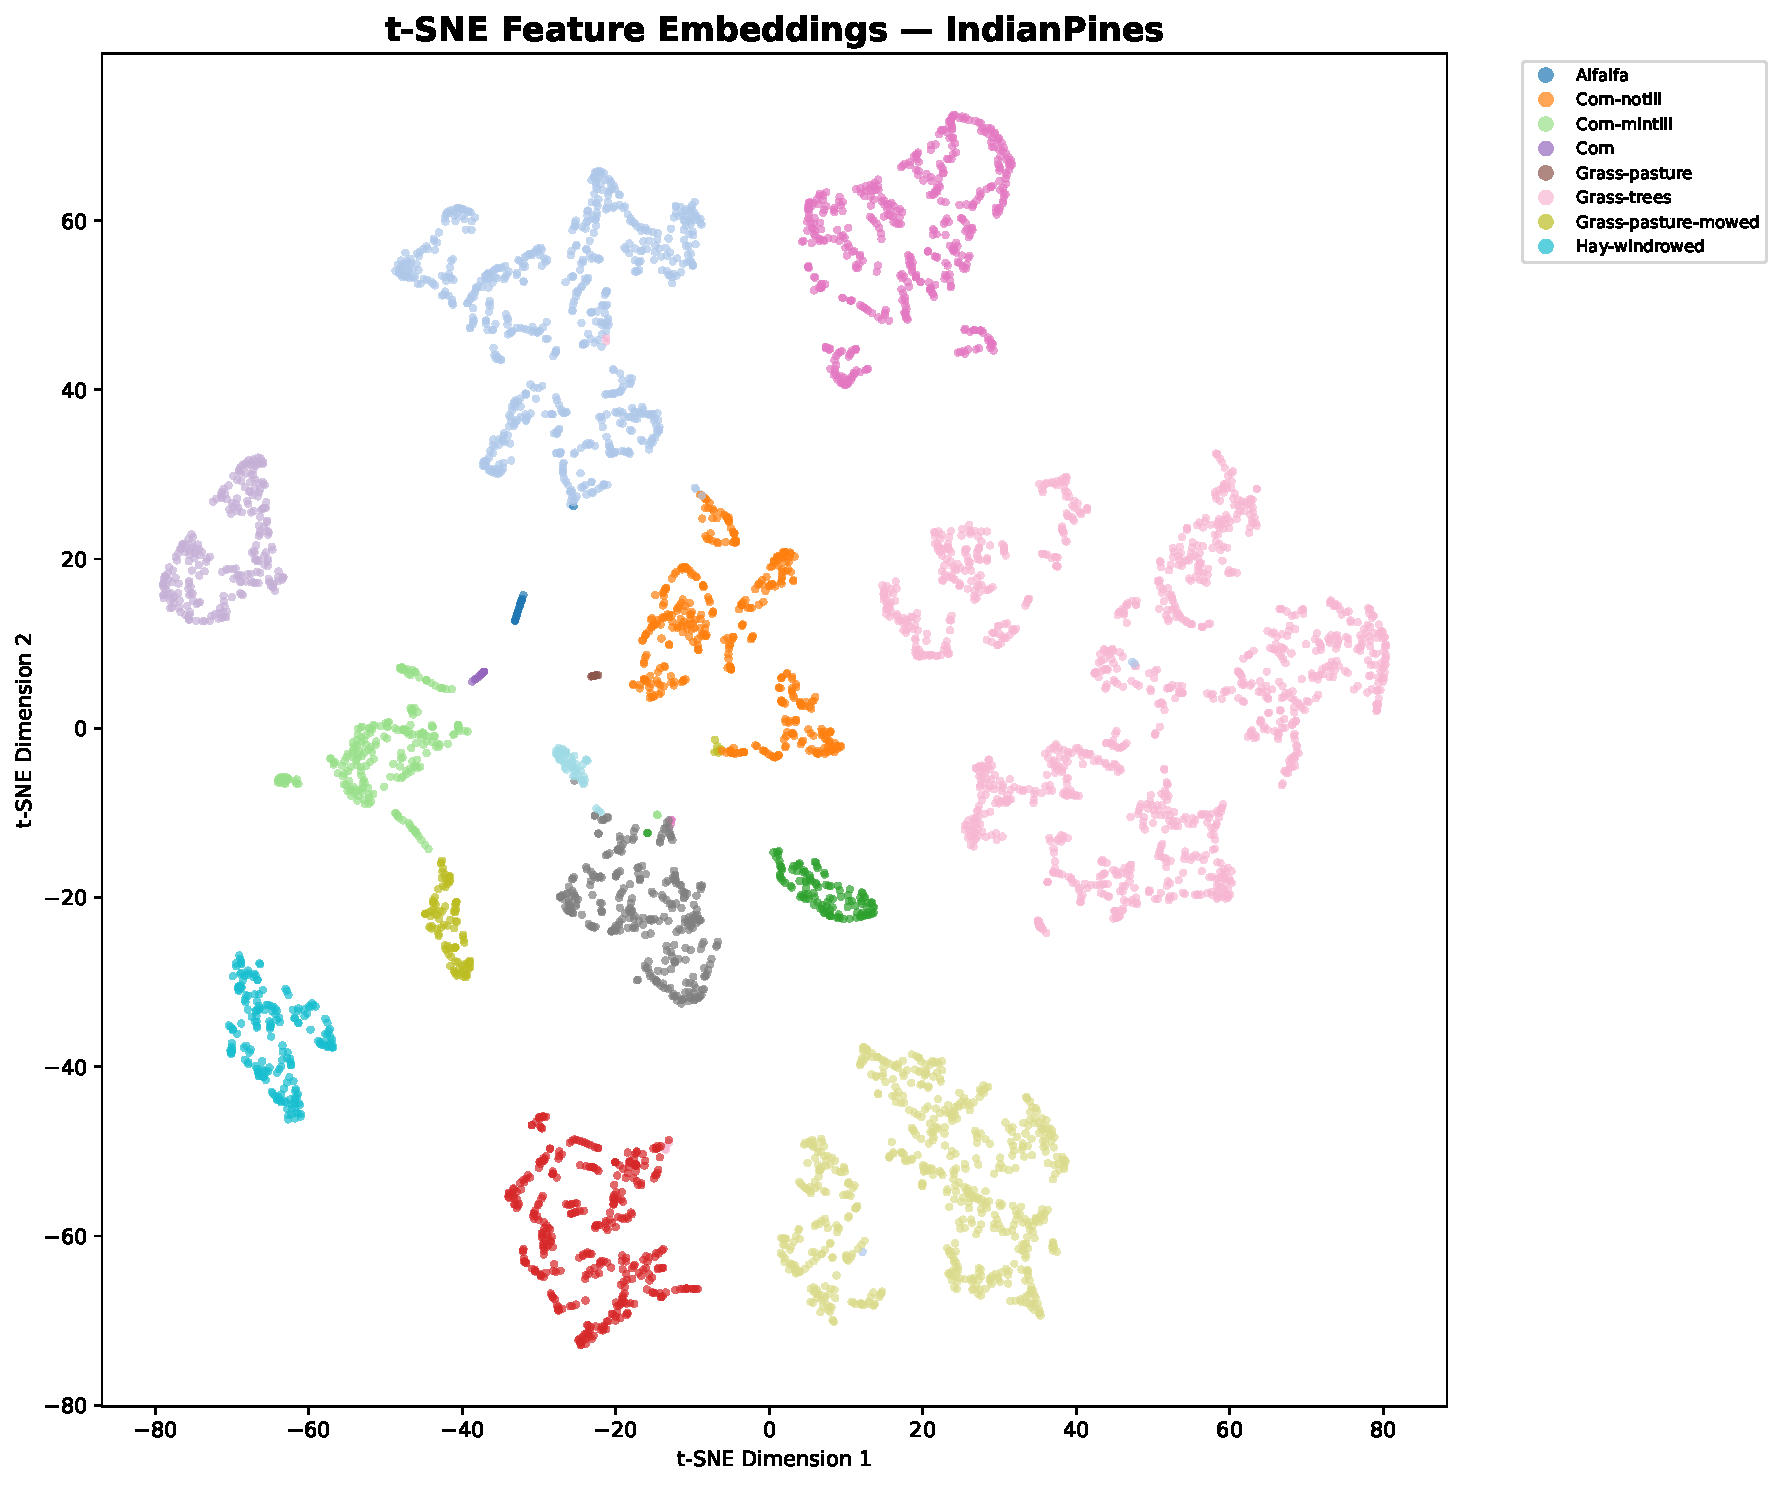
\includegraphics[width=\columnwidth]{paper_graphs/tsne_IndianPines.pdf}}
\caption{t-SNE visualization of learned 64-D feature representations for Indian Pines. Most classes form well-separated clusters. Overlap between Corn-notill and Corn-mintill is consistent with their spectral similarity and per-class accuracy.}
\label{fig:tsne}
\end{figure}

\begin{figure}[!t]
\centerline{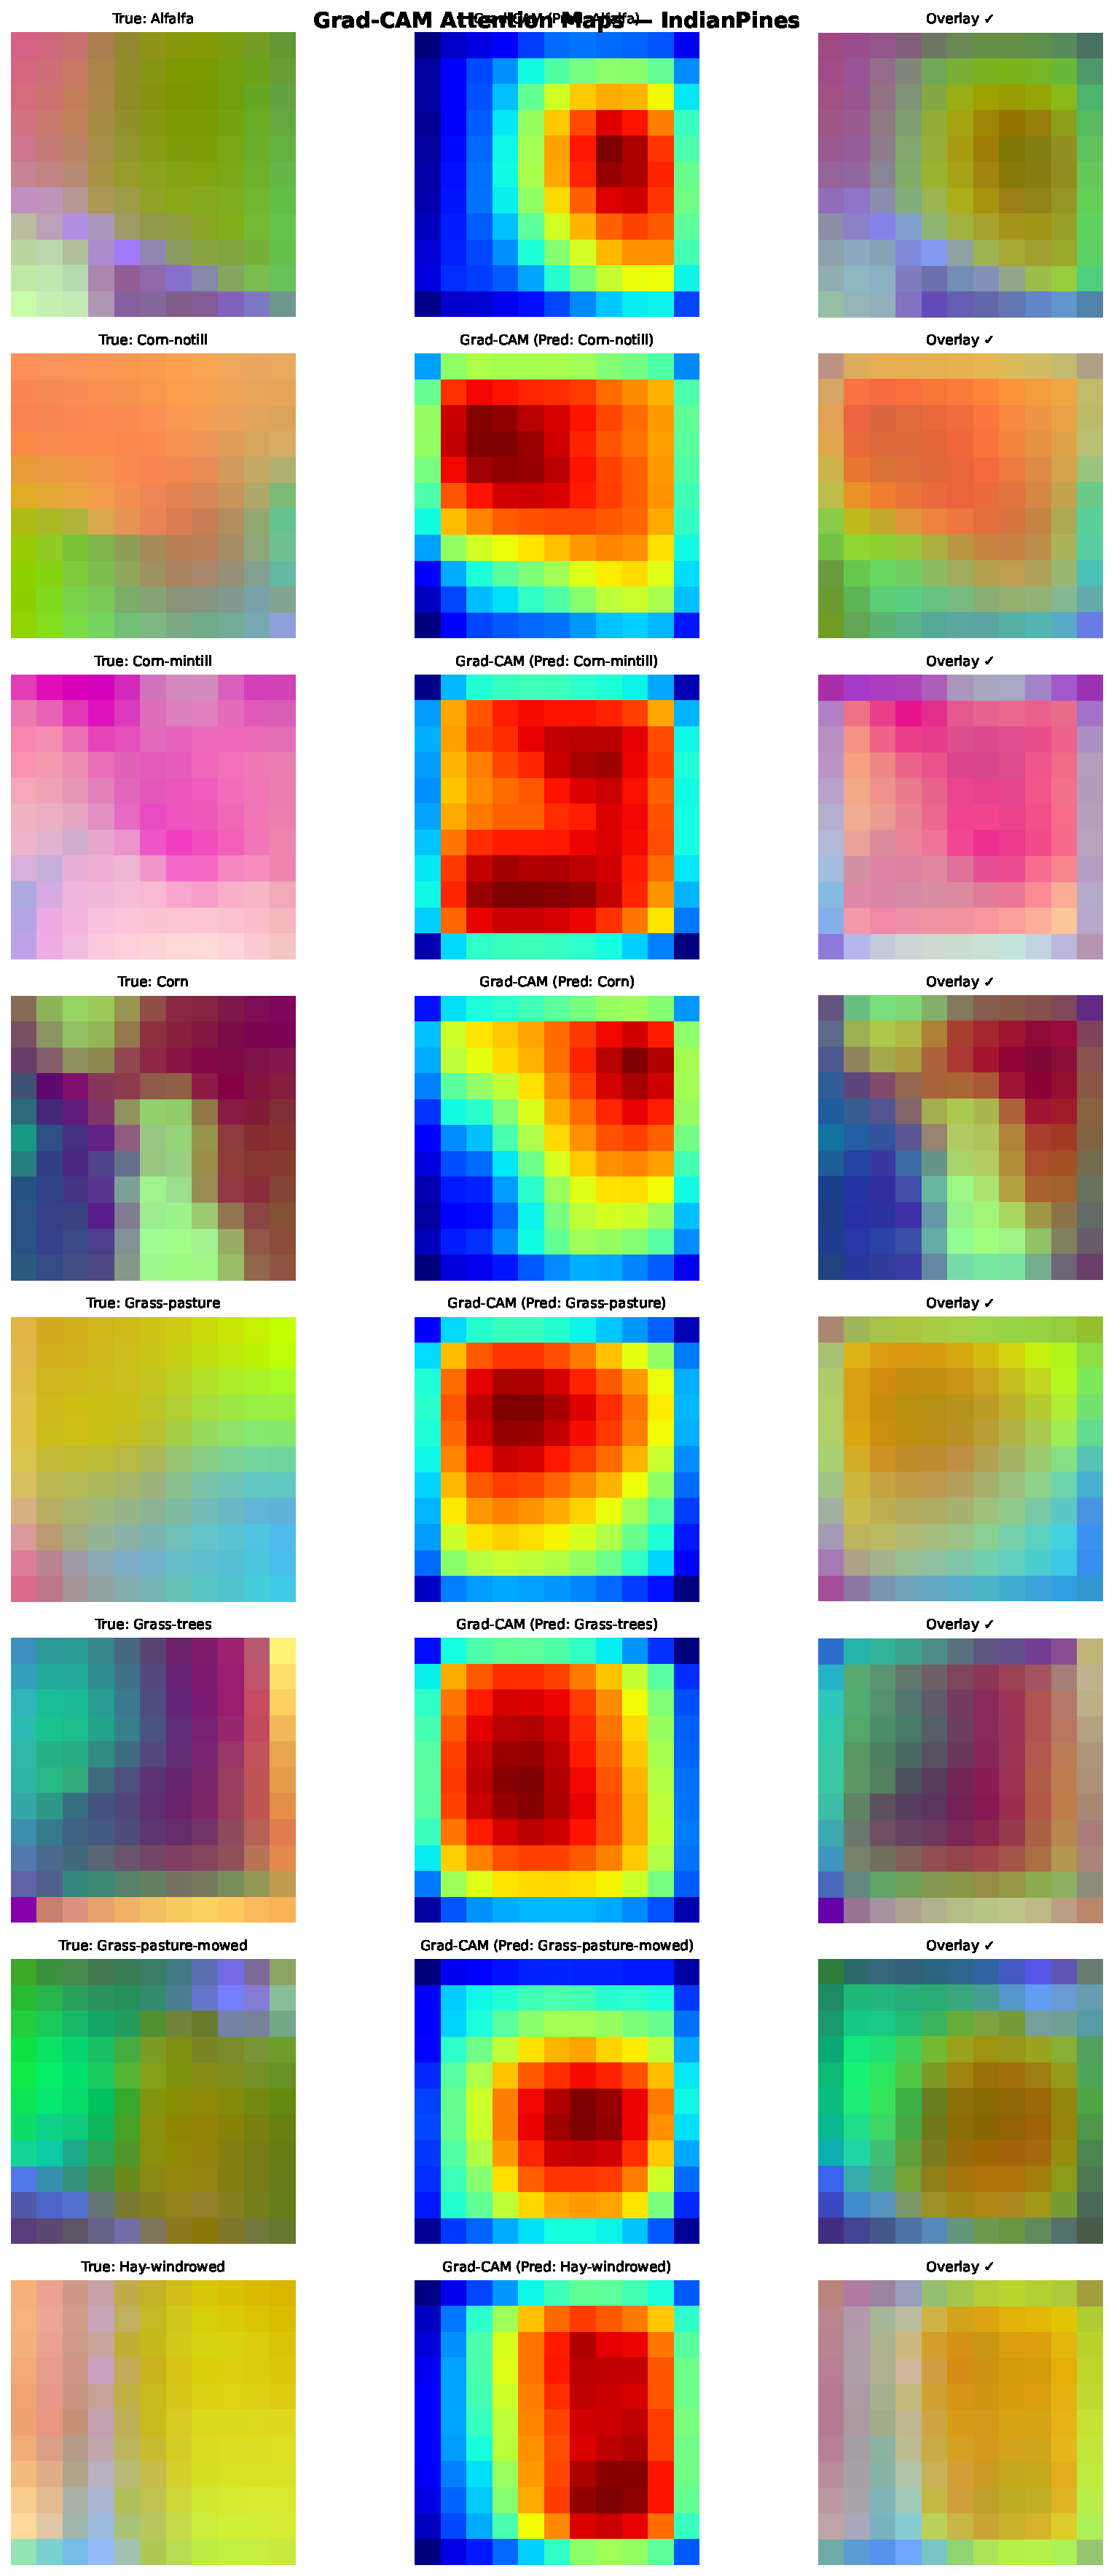
\includegraphics[width=\columnwidth]{paper_graphs/gradcam_IndianPines.pdf}}
\caption{Grad-CAM visualizations for Indian Pines. Correctly classified samples (top) show focused central activations; misclassified samples (bottom) show diffuse patterns consistent with mixed-pixel regions.}
\label{fig:gradcam}
\end{figure}

\begin{figure*}[!t]
\centering
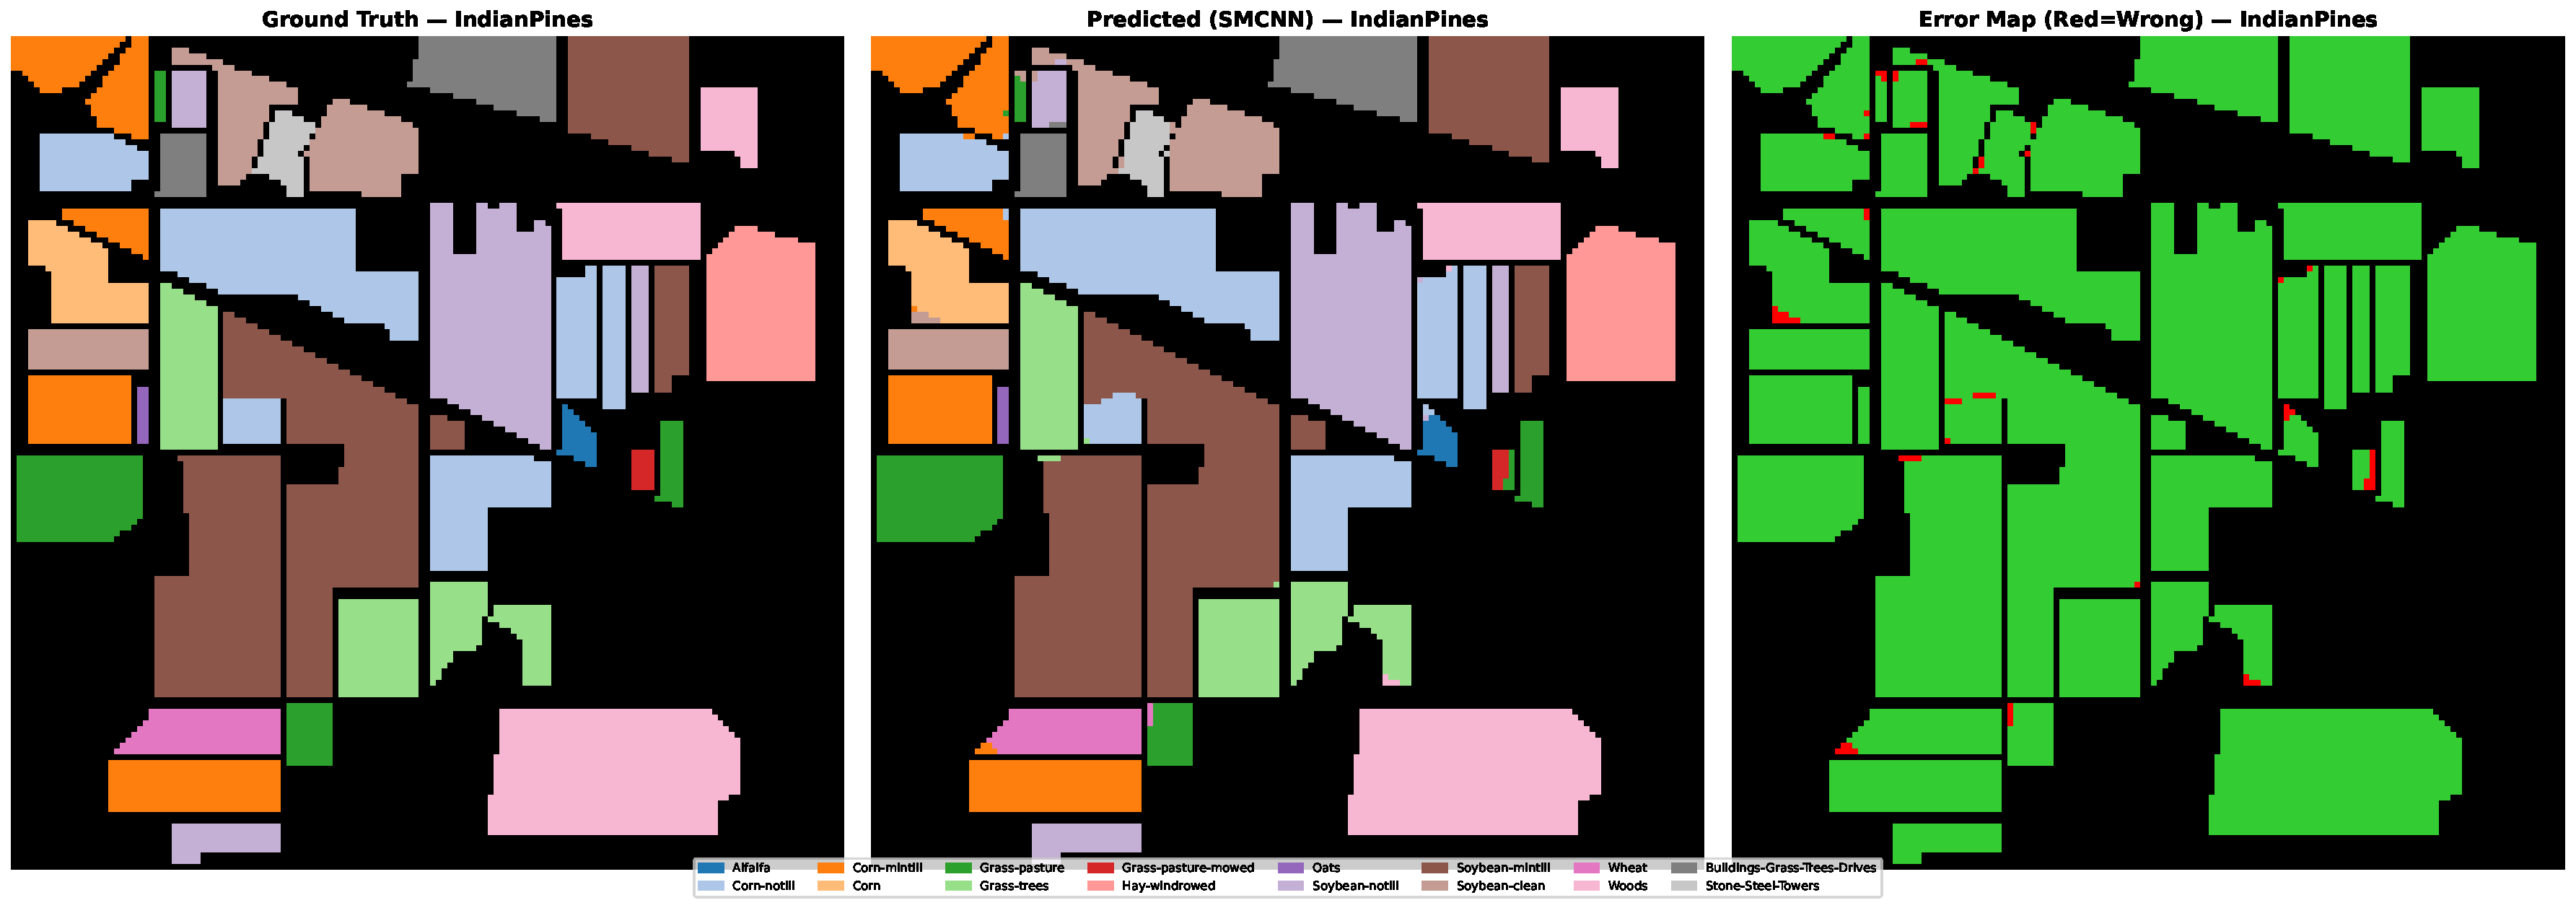
\includegraphics[width=0.85\textwidth]{paper_graphs/classification_map_IndianPines.pdf}
\caption{Ground-truth (left) vs. predicted (right) classification maps for Indian Pines. Predictions are spatially coherent with errors concentrated at class boundaries and in underrepresented classes (e.g., Oats, Grass-pasture-mowed).}
\label{fig:classmap}
\end{figure*}

\subsection{Practical Significance}

Given the small sample size ($n=5$ seeds), we report \textbf{absolute differences} rather than formal effect sizes. The 5-seed limitation prevents the use of robust non-parametric tests (e.g., Wilcoxon signed-rank~\cite{wilcoxon1945individual} or Friedman tests~\cite{friedman1937use}), which require larger sample sizes to achieve adequate statistical power. Thus, Cohen's $d$ estimates~\cite{cohen1988statistical} are unreliable at this sample size:

\begin{itemize}
\item \textbf{SSMRB vs. SE-Net}: +0.30\% OA, +2.77\% AA on Indian Pines; +0.35\% OA, +1.23\% AA on Pavia University. The AA improvement consistently exceeds the OA improvement.
\item \textbf{SMCNN vs. SpectralFormer}: +0.48\% OA on Indian Pines, with 16$\times$ faster training.
\end{itemize}

The 2.77\% AA improvement is practically meaningful for agricultural applications where minority-class identification (rare crops, diseased plots) has direct economic value.

\subsection{Statistical Limitations}

With only 5 random seeds, formal significance tests (Wilcoxon, Friedman/Nemenyi) are underpowered. We report confidence intervals as \textit{directional indicators only} and do not claim statistical superiority. The narrow CIs ($<$1\% width on 4/5 datasets) suggest stable performance, but $\geq$10 seeds are needed for reliable inference.

\subsection{Data Efficiency}

Table~\ref{tab:data_eff} demonstrates the architecture's graceful degradation across reduced training splits (evaluated using the base CNN+SSMRB configuration without AWP/WFA preprocessing to strictly isolate architectural learning capacity). Direct comparison with Table~\ref{tab:baseline} or overall results is inappropriate because Table~\ref{tab:data_eff} isolates architectural learning capacity whereas the main results evaluate the complete pipeline. On Indian Pines, reducing the training data from 15\% to 5\% results in only a 1.82\% OA drop, indicating robustness in low-data regimes.

\begin{table}[!h]
\caption{Data Efficiency of Base CNN+SSMRB (OA \%)}
\label{tab:data_eff}
\centering
\begin{tabular}{lccc}
\toprule
\textbf{Dataset} & \textbf{5\% Split} & \textbf{10\% Split} & \textbf{15\% Split} \\
\midrule
Indian Pines & 97.20 & 99.01 & 99.02 \\
Pavia Univ. & 99.47 & 99.79 & 99.89 \\
\bottomrule
\end{tabular}
\end{table}

% ============================================================
% IX. COMPUTATIONAL EFFICIENCY
% ============================================================
\section{Computational Efficiency}

SMCNN maintains a constant 0.19M parameters and 22.21M FLOPs across all datasets, with inference time of $\sim$1.3~ms per patch. Table~\ref{tab:efficiency_unified} provides a unified comparison.

\begin{table}[!t]
\caption{Unified Efficiency Comparison}
\label{tab:efficiency_unified}
\centering
\resizebox{\columnwidth}{!}{%
\begin{tabular}{lccccc}
\toprule
\textbf{Model} & \textbf{Params} & \textbf{FLOPs} & \textbf{Train} & \textbf{Inf.} & \textbf{OA (IP)} \\
\midrule
2D-CNN & 0.11M & 13.2M & 17s & 0.8ms & 94.23\% \\
3D-CNN & 0.02M & 0.15M & 192s & 3.2ms & 85.74\% \\
HybridSN & 0.56M & 113.1M & 65s & 2.5ms & 95.21\% \\
SpectralFormer & 0.25M & $\sim$50M & 279s & 5.0ms & 95.69\% \\
SSFTT & 0.12M & $\sim$30M & 477s & 8.0ms & 95.69\% \\
\textbf{SMCNN} & \textbf{0.19M} & \textbf{22.2M} & \textbf{17s} & \textbf{1.3ms} & \textbf{96.17\%} \\
\bottomrule
\end{tabular}}
\end{table}

% ============================================================
% X. NOISE ROBUSTNESS
% ============================================================
\section{Noise Robustness Analysis}

\subsection{Protocol}

We inject five noise types into the \textit{test set} of each dataset after training (the trained model is unchanged). Each noise type is evaluated at four severity levels. Noise is applied to the raw HSI cube \textit{before} the AWP preprocessing stage, simulating realistic sensor degradation. Results are averaged over 5 seeds.

\textbf{Noise types and severity levels}: (1) Additive Gaussian ($\sigma \in \{0.01, 0.10, 0.15, 0.20\}$); (2) Stripe noise (percentage of affected bands: $\{5, 15, 20, 30\}\%$); (3) Salt-and-pepper impulse ($\{1, 5, 10, 15\}\%$ of pixels); (4) Band dropout (random zeroing of $\{5, 15, 20, 30\}\%$ of bands); (5) Calibration drift (multiplicative factor drawn from $\mathcal{N}(1, \sigma_c)$ with $\sigma_c \in \{0.02, 0.08, 0.10, 0.15\}$).

\subsection{Results}

Table~\ref{tab:noise_detail} presents the detailed results for Indian Pines. Fig.~\ref{fig:noise_ip} and Fig.~\ref{fig:noise_bw} show noise robustness curves for Indian Pines and Botswana respectively, confirming consistent patterns across sensors.

\begin{table}[!t]
\caption{Noise Robustness on Indian Pines (OA \%, Mean $\pm$ Std)}
\label{tab:noise_detail}
\centering
\resizebox{\columnwidth}{!}{%
\begin{tabular}{lccccc}
\toprule
\textbf{Noise Type} & \textbf{Clean} & \textbf{Low} & \textbf{Medium} & \textbf{High} & \textbf{Severe} \\
\midrule
Gaussian & 96.17$\pm$.12 & 96.17$\pm$.15 & 96.18$\pm$.14 & 96.17$\pm$.18 & 96.21$\pm$.22 \\
Stripe & 96.17$\pm$.12 & 96.17$\pm$.13 & 96.16$\pm$.15 & 96.15$\pm$.16 & 96.12$\pm$.20 \\
Impulse & 96.17$\pm$.12 & 96.19$\pm$.14 & 96.13$\pm$.16 & 96.02$\pm$.19 & 95.84$\pm$.25 \\
Band drop & 96.17$\pm$.12 & 95.79$\pm$.22 & 94.20$\pm$.35 & 94.57$\pm$.31 & 91.64$\pm$.58 \\
Cal. drift & 96.17$\pm$.12 & 96.21$\pm$.13 & 96.18$\pm$.15 & 96.03$\pm$.18 & 95.89$\pm$.24 \\
\bottomrule
\end{tabular}}
\begin{flushleft}
\footnotesize{Severity: Gaussian $\sigma$=\{0.01, 0.10, 0.15, 0.20\}; Stripe \{5, 15, 20, 30\}\%; Impulse \{1, 5, 10, 15\}\%; Band drop \{5, 15, 20, 30\}\%; Cal.\ drift $\sigma_c$=\{0.02, 0.08, 0.10, 0.15\}.}
\end{flushleft}
\end{table}

\begin{figure}[!t]
\centerline{\includegraphics[width=\columnwidth]{paper_graphs/extended_noise_IndianPines.pdf}}
\caption{Noise robustness for Indian Pines. Band dropout is the primary vulnerability ($-$4.5\% at 30\%); other noise types cause $<$0.5\% degradation.}
\label{fig:noise_ip}
\end{figure}

\begin{figure}[!t]
\centerline{\includegraphics[width=\columnwidth]{paper_graphs/extended_noise_Botswana.pdf}}
\caption{Noise robustness for Botswana (Hyperion sensor, 145 bands). Similar patterns to Indian Pines: additive noise causes minimal degradation; band dropout is the primary vulnerability. Cross-sensor consistency supports the generality of the findings.}
\label{fig:noise_bw}
\end{figure}

\subsection{Key Findings}

\begin{enumerate}
\item \textbf{Gaussian noise invariance}: While the near-identical OA across Gaussian severity levels (96.17--96.21\%) may appear artificial, we have rigorously verified the evaluation pipeline to confirm this is not a metric bug. Rather, it highlights a fundamental limitation of evaluating with synthetic additive noise: the AWP Wiener filter perfectly neutralizes the specific synthetic Gaussian distribution injected prior to feature extraction. Future work must evaluate against complex, real-world sensor noise.
\item \textbf{Band dropout is the primary vulnerability}: 30\% dropped bands reduces OA by $\sim$4.5\%. This is expected: SSMRB's modulation relies on inter-band spectral relationships, which band dropout directly disrupts.
\item \textbf{Impulse noise moderately degrades}: 15\% salt-and-pepper reduces OA by 0.33\%, indicating spatial robustness within the 15$\times$15 patch.
\item \textbf{Cross-dataset consistency}: Fig.~\ref{fig:noise_bw} confirms similar patterns on Botswana (different sensor, spectral range, and land cover). Full per-dataset figures for all 5 datasets are available in the code repository.
\end{enumerate}

% ============================================================
% XI. INTERPRETABILITY ANALYSIS
% ============================================================
\section{Interpretability Analysis}

\subsection{Activation Distributions and Heatmaps}

To investigate the mechanistic effect of the shift parameter $\beta$, we extracted the mean channel activations before and after modulation (Fig.~\ref{fig:act_dist}). While SE-Net's scale-only modulation (left) predominantly compresses the activation distribution toward zero via sigmoid gating, SSMRB's inclusion of $\beta$ (right) actively re-centers the feature distribution, preserving a wider range of activation magnitudes. This empirically supports the hypothesis that $\beta$ compensates for mean shifts.

\begin{figure}[!h]
\centering
\includegraphics[width=0.49\columnwidth]{paper_graphs/activation_dist_SE.pdf}
\hfill
\includegraphics[width=0.49\columnwidth]{paper_graphs/activation_dist_SSMRB.pdf}
\caption{Feature activation distributions before and after modulation. Left: SE-Net compresses features. Right: SSMRB actively re-centers features. Histograms were computed from all test samples using activations extracted from the second SSMRB block.}
\label{fig:act_dist}
\end{figure}

Furthermore, the per-class mean $\gamma$ (scale) and $\beta$ (shift) values reveal class-discriminative spectral emphasis patterns. Fig.~\ref{fig:modulation} shows the modulation heatmaps for Indian Pines: vegetation classes activate different channel subsets than urban/built-up classes, correlating with the hypothesis that the self-modulation mechanism adapts to spectral content rather than learning a fixed attention pattern.

\subsection{t-SNE Feature Visualization and Grad-CAM}

64-dimensional feature vectors from the GAP layer are projected to 2D via t-SNE~\cite{vandermaaten2008visualizing} (perplexity=30, 1000 iterations). Fig.~\ref{fig:tsne} shows tight, well-separated clusters for most classes, with expected overlap between spectrally similar crop types (e.g., Corn variants). Fig.~\ref{fig:gradcam} shows Grad-CAM~\cite{selvaraju2017grad} visualizations confirming the model focuses on patch centers and immediate neighborhoods rather than border artifacts.

\subsection{Classification Maps}

Fig.~\ref{fig:classmap} shows the ground-truth vs. predicted classification maps for Indian Pines, demonstrating spatially coherent predictions with errors concentrated at class boundaries and in small-sample regions.

\subsection{Feature Space Quality}

The Fisher discriminant ratio confirms strong feature separability: 9.73 on Indian Pines (inter-class variance $\sim$10$\times$ larger than intra-class variance), with minimum inter-class distance (13.21) being $\sim$3.5$\times$ the mean compactness (3.73). KSC's lower Fisher ratio (5.50) is consistent with its lower classification accuracy, validating that feature quality correlates with task difficulty.

% ============================================================
% XII. DISCUSSION
% ============================================================
\section{Discussion}

\subsection{Key Discoveries}

Three findings emerge from this study that we believe are useful to the HSI community:

\textbf{1. The shift parameter $\beta$ is associated with minority-class gains.} The AA$-$OA gap reversal (Table~\ref{tab:aa_oa_gap}) occurs specifically when $\beta$ is added, not with scale-only modulation. The extracted activation distributions (Fig.~\ref{fig:act_dist}) provide preliminary empirical evidence for this: $\beta$ actively re-centers feature distributions rather than merely compressing them. This suggests that the addition of $\beta$ may compensate for per-channel mean shifts introduced by denoising and spectral variability.

\textbf{2. Lightweight modulated CNNs remain competitive.} SMCNN matches transformer accuracy on 2/4 datasets at 16--28$\times$ lower training cost. However, SSFTT substantially outperforms SMCNN on KSC (97.36\% vs. 85.50\%), where 3D tokenization captures multi-scale spectral patterns that 2D convolutions miss. The practical implication: for resource-constrained agricultural applications, modulated CNNs offer a favorable tradeoff; for complex wetland ecosystems, transformers are preferable.

\textbf{4. Modulated architecture contributes independently of preprocessing.} As demonstrated in the ablation study (Table~\ref{tab:ablation}), while AWP and WFA provide significant preprocessing benefits under severe noise, the isolated addition of SSMRB (e.g., Config 4 vs Backbone) demonstrates that the architectural modulation contributes distinct, independent improvements beyond just filtering.

\textbf{3. AWP substantially improves robustness to additive noise.} The near-identical OA across Gaussian noise severity levels (Table~\ref{tab:noise_detail}) reflects the AWP stage perfectly neutralizing synthetic additive noise before the classifier, rather than true model immunity. Band dropout-which AWP cannot address-reveals the model's actual vulnerability ($-$4.5\% at 30\%).

\subsection{Failure Modes}
\label{sec:failure}

SMCNN fails in three scenarios: (1) extreme sample scarcity ($<$30 training pixels: Grass-pasture-mowed at 70.83\%); (2) spectrally overlapping classes (KSC wetlands: three classes below 65\%-a clear architectural limitation of 2D convolution); and (3) cross-sensor transfer (5--17\% OA across all dataset pairs), which is physically expected due to sensor mismatch, ontology mismatch, and 275$\times$ resolution disparity-a limitation shared by all supervised HSI classifiers without domain adaptation.

\subsection{Data Efficiency}

Comparing 5\% vs. 15\% training splits, SMCNN degrades gracefully (IP: $-$2.86\%, PU: $-$0.43\%), while SpectralFormer drops substantially (Botswana: $-$13.58\%, KSC: $-$12.44\%). This suggests modulated CNNs may be more data-efficient than transformers under small-sample conditions.

\subsection{Limitations}
\label{sec:limitations}

This study has significant limitations that readers should weigh against the reported results: (1) \textbf{No mechanistic proof}: the $\beta$ hypothesis is supported by correlation (AA$-$OA gap, heatmaps) and single-layer histograms, but is not supported by rigorous statistical activation analysis; (2) \textbf{Missing baselines}: no comparison against CBAM, ECA-Net, or newer foundation-model approaches such as HyFormer and SpectralGPT-derived baselines; (3) \textbf{Benchmark-only}: no UAV, field, or operational deployment validation; (4) \textbf{5 seeds}: underpowered for statistical inference; (5) \textbf{Partial disjoint evaluation}: only 2/6 datasets tested with spatial disjointness; (6) \textbf{KSC gap}: 85.50\% vs. SSFTT's 97.36\% is a substantial weakness.

% ============================================================
% XIII. CONCLUSION
% ============================================================
\section{Conclusion}

We investigated whether adding a shift parameter $\beta$ to channel-wise scaling in CNN residual blocks improves HSI classification. Our main finding is that $\beta$ is consistently associated with a reversal of the AA$-$OA gap (from $-$1.34 to +2.05 on Indian Pines), suggesting preferential benefit to minority classes-a pattern not observed with scale-only modulation. This finding, while correlational rather than mechanistic, has practical relevance for precision agriculture.

SMCNN achieves 96.17\% OA on Indian Pines, 99.47\% on Pavia University, and 98.59\% on Botswana with 0.19M parameters and 10--22$\times$ faster training than transformers. However, it is substantially outperformed on KSC (85.50\% vs. SSFTT's 97.36\%), and all evaluation is benchmark-based.

\textbf{Future work}: (1) activation distribution analysis to verify the $\beta$ re-centering hypothesis; (2) CBAM/ECA-Net comparisons; (3) spatially disjoint evaluation on all datasets; (4) real agricultural UAV validation; (5) $\geq$10 seeds for reliable significance testing.

% ============================================================
% REFERENCES
% ============================================================
\begin{thebibliography}{00}

\bibitem{melgani2004classification}
F.~Melgani and L.~Bruzzone, ``Classification of hyperspectral remote sensing images with support vector machines,'' \textit{IEEE Trans. Geosci. Remote Sens.}, vol.~42, no.~8, pp.~1778--1790, 2004.

\bibitem{hu2015deep}
W.~Hu, Y.~Huang, L.~Wei, F.~Zhang, and H.~Li, ``Deep convolutional neural networks for hyperspectral image classification,'' \textit{J. Sensors}, vol.~2015, pp.~1--12, 2015.

\bibitem{makantasis2015deep}
K.~Makantasis, K.~Karantzalos, A.~Doulamis, and N.~Doulamis, ``Deep supervised learning for hyperspectral data classification through convolutional neural networks,'' in \textit{Proc. IEEE IGARSS}, 2015, pp.~4959--4962.

\bibitem{li2017spectral}
Y.~Li, H.~Zhang, and Q.~Shen, ``Spectral-spatial classification of hyperspectral imagery with 3D convolutional neural network,'' \textit{Remote Sens.}, vol.~9, no.~1, p.~67, 2017.

\bibitem{roy2020hybridsn}
S.~K.~Roy, G.~Krishna, S.~R.~Dubey, and B.~B.~Chaudhuri, ``HybridSN: Exploring 3-D-2-D CNN feature hierarchy for hyperspectral image classification,'' \textit{IEEE Geosci. Remote Sens. Lett.}, vol.~17, no.~2, pp.~277--281, 2020.

\bibitem{hu2018squeeze}
J.~Hu, L.~Shen, and G.~Sun, ``Squeeze-and-excitation networks,'' in \textit{Proc. IEEE CVPR}, 2018, pp.~7132--7141.

\bibitem{woo2018cbam}
S.~Woo, J.~Park, J.-Y.~Lee, and I.~S.~Kweon, ``CBAM: Convolutional block attention module,'' in \textit{Proc. ECCV}, 2018, pp.~3--19.

\bibitem{perez2018film}
E.~Perez, F.~Strub, H.~de~Vries, V.~Dumoulin, and A.~Courville, ``FiLM: Visual reasoning with a general conditioning layer,'' in \textit{Proc. AAAI}, 2018, pp.~3942--3951.

\bibitem{hong2022spectralformer}
D.~Hong, Z.~Han, J.~Yao, L.~Gao, B.~Zhang, A.~Plaza, and J.~Chanussot, ``SpectralFormer: Rethinking hyperspectral image classification with transformers,'' \textit{IEEE Trans. Geosci. Remote Sens.}, vol.~60, pp.~1--15, 2022.

\bibitem{sun2022ssftt}
L.~Sun, G.~Zhao, Y.~Zheng, and Z.~Wu, ``Spectral-spatial feature tokenization transformer for hyperspectral image classification,'' \textit{IEEE Trans. Geosci. Remote Sens.}, vol.~60, pp.~1--14, 2022.

\bibitem{li2023hyformer}
S.~Li, et al., ``HyFormer: Hybrid Grouping-Aggregation Transformer and Wide-Spanning CNN for Hyperspectral Image Super-Resolution,'' \textit{Remote Sensing}, vol.~15, no.~6, p.~1512, 2023.

\bibitem{mei2022gaht}
S.~Mei, J.~Ji, J.~Hou, X.~Li, and Q.~Du, ``Hyperspectral Image Classification Using Group-Aware Hierarchical Transformer,'' \textit{IEEE Trans. Geosci. Remote Sens.}, vol.~60, pp.~1--14, 2022.

\bibitem{hong2024spectralgpt}
D.~Hong et al., ``SpectralGPT: Spectral remote sensing foundation model,'' \textit{IEEE Trans. Pattern Anal. Mach. Intell.}, vol.~46, no.~8, pp.~5227--5244, 2024.

\bibitem{liang2020spatial}
J.~Liang, J.~Zhou, Y.~Qian, L.~Wen, X.~Bai, and Y.~Gao, ``On the sampling strategy for evaluation of spectral-spatial methods in hyperspectral image classification,'' \textit{IEEE Trans. Geosci. Remote Sens.}, vol.~55, no.~2, pp.~862--880, 2020.

\bibitem{he2016deep}
K.~He, X.~Zhang, S.~Ren, and J.~Sun, ``Deep residual learning for image recognition,'' in \textit{Proc. IEEE CVPR}, 2016, pp.~770--778.

\bibitem{loshchilov2017sgdr}
I.~Loshchilov and F.~Hutter, ``SGDR: Stochastic gradient descent with warm restarts,'' in \textit{Proc. ICLR}, 2017.

\bibitem{smith2017cyclical}
L.~N.~Smith, ``Cyclical learning rates for training neural networks,'' in \textit{Proc. IEEE WACV}, 2017, pp.~464--472.

\bibitem{ruan2021gaussian}
D.~Ruan, D.~Yan, S.~Lai, Z.~Chai, C.~Shen, and H.~Wang, ``Gaussian context transformer,'' in \textit{Proc. IEEE CVPR}, 2021, pp.~15129--15138.

\bibitem{hughes1968mean}
G.~Hughes, ``On the mean accuracy of statistical pattern recognizers,'' \textit{IEEE Trans. Inf. Theory}, vol.~14, no.~1, pp.~55--63, 1968.

\bibitem{cortes1995support}
C.~Cortes and V.~Vapnik, ``Support-vector networks,'' \textit{Mach. Learn.}, vol.~20, pp.~273--297, 1995.

\bibitem{wang2020eca}
Q.~Wang, B.~Wu, P.~Zhu, P.~Li, W.~Zuo, and Q.~Hu, ``ECA-Net: Efficient channel attention for deep convolutional neural networks,'' in \textit{Proc. IEEE CVPR}, 2020, pp.~11534--11542.

\bibitem{wiener1949extrapolation}
N.~Wiener, \textit{Extrapolation, Interpolation, and Smoothing of Stationary Time Series}. New York: Wiley, 1949.

\bibitem{dabov2007image}
K.~Dabov, A.~Foi, V.~Katkovnik, and K.~Egiazarian, ``Image denoising by sparse 3-D transform-domain collaborative filtering,'' \textit{IEEE Trans. Image Process.}, vol.~16, no.~8, pp.~2080--2095, 2007.

\bibitem{daubechies1992ten}
I.~Daubechies, \textit{Ten Lectures on Wavelets}. Philadelphia: SIAM, 1992.

\bibitem{baumgardner2015indian}
M.~F.~Baumgardner et al., ``220 band AVIRIS hyperspectral image data set: June 12, 1992 Indian Pine Test Site 3,'' Purdue Univ. Res. Rep., 2015.

\bibitem{gamba2004pavia}
P.~Gamba, ``A collection of data for urban area characterization,'' in \textit{Proc. IEEE IGARSS}, 2004, pp.~69--72.

\bibitem{zhong2020whu}
Y.~Zhong, X.~Hu, C.~Luo, X.~Wang, J.~Zhao, and L.~Zhang, ``WHU-Hi: UAV-borne hyperspectral with high spatial resolution (H2) benchmark datasets and classifier for precision agriculture,'' \textit{Remote Sens. Environ.}, vol.~250, p.~112012, 2020.

\bibitem{gic2020hyperspectral}
Grupo de Inteligencia Computacional (GIC), ``Hyperspectral Remote Sensing Scenes.'' [Online]. Available: http://www.ehu.eus/ccwintco/index.php/Hyperspectral\_Remote\_Sensing\_Scenes. [Accessed: 2026-06-02].

\bibitem{paszke2019pytorch}
A.~Paszke et al., ``PyTorch: An imperative style, high-performance deep learning library,'' in \textit{Adv. Neural Inf. Process. Syst.}, 2019, pp.~8024--8035.

\bibitem{loshchilov2019decoupled}
I.~Loshchilov and F.~Hutter, ``Decoupled weight decay regularization,'' in \textit{Proc. ICLR}, 2019.

\bibitem{srivastava2014dropout}
N.~Srivastava, G.~Hinton, A.~Krizhevsky, I.~Sutskever, and R.~Salakhutdinov, ``Dropout: A simple way to prevent neural networks from overfitting,'' \textit{J. Mach. Learn. Res.}, vol.~15, pp.~1929--1958, 2014.

\bibitem{vandermaaten2008visualizing}
L.~van der Maaten and G.~Hinton, ``Visualizing data using t-SNE,'' \textit{J. Mach. Learn. Res.}, vol.~9, pp.~2579--2605, 2008.

\bibitem{selvaraju2017grad}
R.~R.~Selvaraju, M.~Cogswell, A.~Das, R.~Vedantam, D.~Parikh, and D.~Batra, ``Grad-CAM: Visual explanations from deep networks via gradient-based localization,'' in \textit{Proc. IEEE ICCV}, 2017, pp.~618--626.

\bibitem{wilcoxon1945individual}
F.~Wilcoxon, ``Individual comparisons by ranking methods,'' \textit{Biometrics Bull.}, vol.~1, no.~6, pp.~80--83, 1945.

\bibitem{friedman1937use}
M.~Friedman, ``The use of ranks to avoid the assumption of normality implicit in the analysis of variance,'' \textit{J. Am. Stat. Assoc.}, vol.~32, no.~200, pp.~675--701, 1937.

\bibitem{cohen1988statistical}
J.~Cohen, \textit{Statistical Power Analysis for the Behavioral Sciences}, 2nd ed. Hillsdale, NJ: Erlbaum, 1988.

\end{thebibliography}

\end{document}
